\begin{figure}
\centering
\begin{tabular}{ccc}
	Maze 
	& $A[0]$ (downward)
	& $A[1]$ (rightward) \\
	\raisebox{-0.5\height}{
		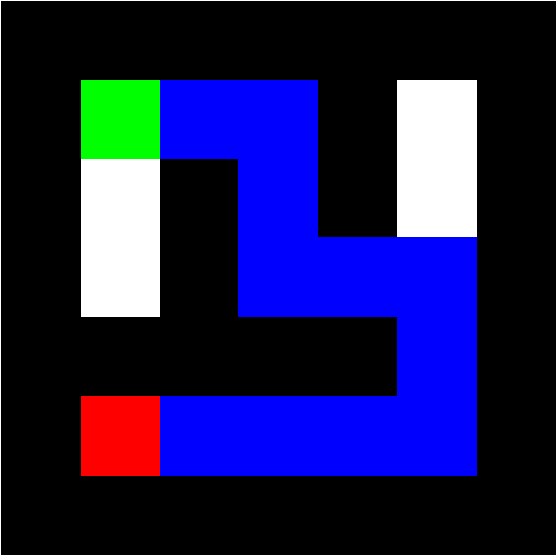
\includegraphics[width=5em]{figures/tex/maze-impl.pdf}
	}
	& \raisebox{-0.5em}{
		\large $\begin{bmatrix}
			1 & 1 & 1 \\
			0 & 0 & 1 \\
			0 & 0 & 0
		\end{bmatrix}$
	}
	& \raisebox{-0.5em}{
		\large $\begin{bmatrix}
			1 & 0 & 0 \\
			0 & 1 & 0 \\
			1 & 1 & 0
		\end{bmatrix}$
	}
\end{tabular}
\caption{
	We describe mazes with the following representation: for a $2$-dimensional lattice with $r$ rows and $c$ columns, we initialize a boolean array $A = \{0, 1\}^{2 \times r \times c}$ which we refer to in the code as a \href{https://understanding-search.github.io/maze-dataset/maze_dataset.html#LatticeMaze.connection_list}{\texttt{connection\_list}}. The value at $A[0,i,j]$ determines whether a \emph{downward} connection exists from node $[i,j]$ to $[i+1, j]$. Likewise, the value at $A[1,i,j]$ determines whether a \emph{rightward} connection to $[i, j+1]$ exists. Thus, we avoid duplication of data about the existence of connections and facilitate fast lookup time, at the cost of requiring additional care with indexing.
}
\label{fig:maze-impl}
\end{figure}